\documentclass{article}
\usepackage[margin=2cm]{geometry}
\usepackage[latin1]{inputenc}
\usepackage{caption}
\usepackage{subcaption}
\usepackage{graphicx}
\usepackage{listings}
\usepackage{color}
\usepackage{textcomp}
\usepackage{float}

\definecolor{aliceblue}{rgb}{0.94, 0.97, 1.0}
\definecolor{almond}{rgb}{0.94, 0.87, 0.8}
\definecolor{asparagus}{rgb}{0.53, 0.66, 0.42}
\definecolor{gainsboro}{rgb}{0.86, 0.86, 0.86}
\definecolor{gray(x11gray)}{rgb}{0.75, 0.75, 0.75}

\lstset{frame=tb,
  aboveskip=3mm,
  belowskip=3mm,
  showstringspaces=false,
  columns=flexible,
  basicstyle={\small\ttfamily},
  numbers=none,
  breaklines=true,
  breakatwhitespace=true,
  tabsize=4,
  language=python
}


\title{Aurora simulation}
\author{Knut Andre G. Prestsveen}

\begin{document}
\maketitle
\section{Abstract}
The motion of charged solar wind particles in Earth's magnetic field was simulated numerically. The Earth's magnetic field was modeled as the field of a magnetic dipole, and the particles equations of motion were solved using a Runge-Kutta routine.

\section{Theory}
\label{theory}
Polar light arises when charged particles from the sun are lead towards the Earth's poles by the force from the magnetic field. The magnetic field of the earth can, with rather good accuracy, be modeled as a dipole field, and the path of solar wind particles are studied by looking at a few protons. More details of magnetic field, forces and dipole can be found in Griffiths.*REF*

To check the accuracy of the calculation energy, or simply the magnitude of the particles velocities, can be checked to see if it remains constant. This is because the magnetic field does zero work on the particles, and since we don't have included any potential, the velocity should stay constant in magnitude and only change direction.

\section{Implementation}
The physical quantities in the simulations where defined by setting the Earth's radius to 10 units of space, and converting the typical speed of solar wind particles to number of simulation space units per unit time. For the dipole strength I was unfortunately not able to find any good way to define its value, and I ended up playing around with it untill the plots looked sensible.

To carry out the simulation three functions were implemented. One for computing the magnetic field from the dipole in a given position in space, one function defining the equation of motion to be solved, and finally one function that simply utilises SciPy's \colorbox{gainsboro}{\lstinline{solve_ivp}} function in order to obtain the particles path and velocities, and returns them. The function definitions are as follows.

\begin{lstlisting}[label=lst:functions]
def B_field(x, y, z): 
    """ Computes B-field from a dipole in position (x,y,x) """
    r = np.maximum(np.sqrt(x**2 + y**2 + z**2), 0.001) # hack to avoid mess inn origo
    dip_dot_r = x*dp_x + y*dp_y + z*dp_z
    B_x = (mu_0/(4*np.pi)) * ( ( (3*x*dip_dot_r)/(r**5) ) - (dp_x)/(r**3) )
    B_y = (mu_0/(4*np.pi)) * ( ( (3*y*dip_dot_r)/(r**5) ) - (dp_y)/(r**3) )
    B_z = (mu_0/(4*np.pi)) * ( ( (3*z*dip_dot_r)/(r**5) ) - (dp_z)/(r**3) )
    B = np.array([B_x, B_y, B_z])
    return B


def ddt_vel_accl(t, y): 
    """ equation of motion to be solved
        Parameters:
            t : time, scalar
            y : position/velocity, vector, [x, y, z, dx/dt, dy/dy, dz/dt]
        Returns:
            [vx, vy, vz, ax, ay, az] : velocity and acceleration at current time t
    """
    velocity = np.array(y[3:])
    B = B_field(y[0], y[1], y[2])
    acceleration = elementary_charge*np.cross(velocity, B)/proton_mass
    return np.concatenate((velocity, acceleration))


def solve_equation_of_motion(ddt_vel_accl, SIM_TIME, INITIAL, dt):
    sol = solve_ivp(ddt_vel_accl, [0, SIM_TIME], INITIAL, max_step=dt)
    path, velocities = sol.y[:3], sol.y[3:]
    return path, velocities
\end{lstlisting}

\section{Results and discussion}

\begin{figure}[h]
    \begin{subfigure}{0.5\textwidth}
        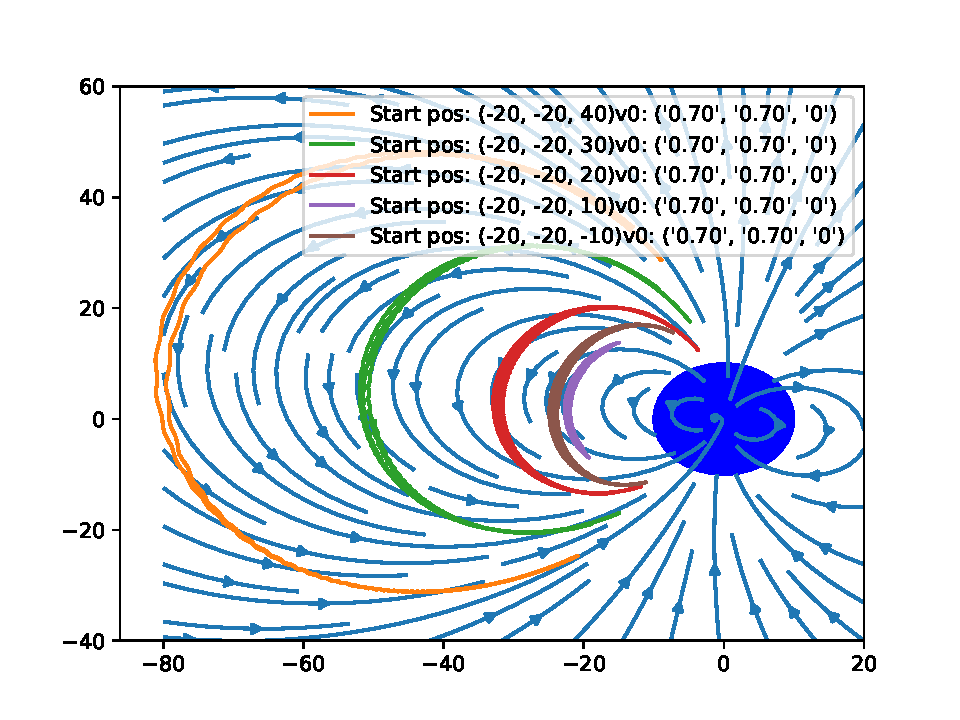
\includegraphics[width=\linewidth]{./media/xz-plane.pdf}
    \end{subfigure}
    \begin{subfigure}{0.5\textwidth}
        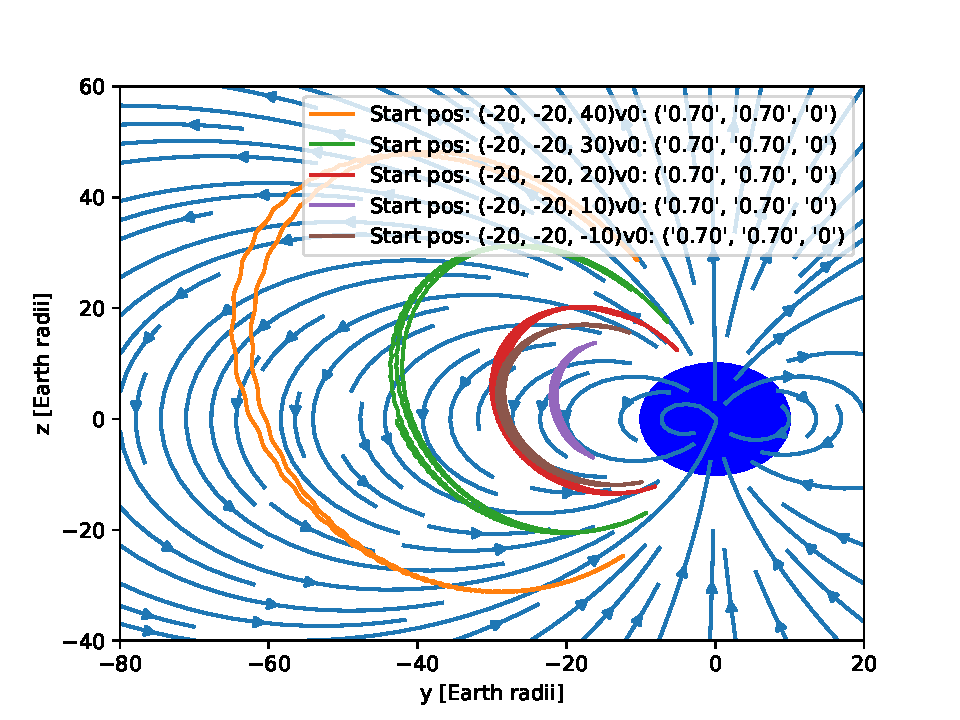
\includegraphics[width=\linewidth]{./media/yz-plane.pdf}
    \end{subfigure}
    \caption{Paths in the xz- and yz planes.}
    \label{paths}
\end{figure}

\begin{figure}
    \begin{subfigure}{0.5\textwidth}
        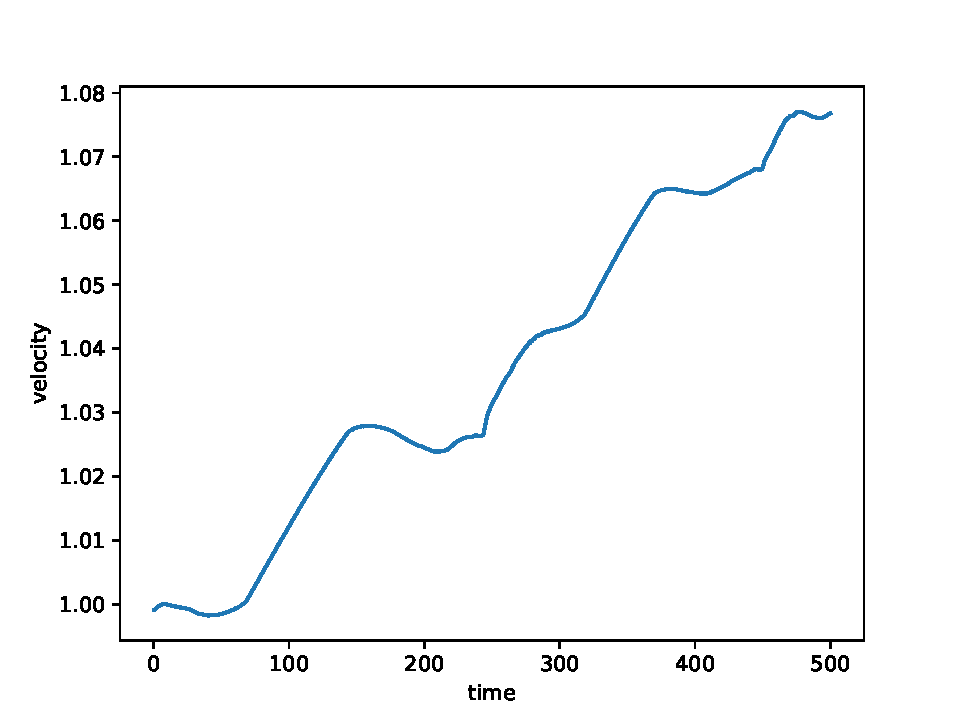
\includegraphics[width=\linewidth]{./media/velocity.pdf}
    \end{subfigure}
    \caption{Magnitude of velocity}
    \label{velocity}
\end{figure}

\noindent
From the figures in \ref{paths} we see that the resulting patterns are spiraling trails towards the northern and southern poles, for the chosen initial velocity, which means they potentially could hit the atmosphere of the Earth and generate aurora. From the electromagnetic theory we know that the force from a magnetic field points perpendicular to bothe the field and the particle's velocity, and therefor a spiralling path is expected for a particle with both an initiall velocity
perpendicular and parallell to the field.

In figure \ref{velocity} we see that the particles velocity varies very little, as it should. Ideally it should be contant according to section \ref{theory}, but some variation occurs beacause of the error from the numerical solver. Since the variation is small however, the numerical precision seems to be quite good.

\end{document}



